\documentclass[aspectratio=43,xcolor={rgb}]{beamer}
\usepackage[utf8]{inputenc}
\usepackage[T1]{fontenc}
\usepackage{lmodern}
\usepackage{graphicx}
\usepackage{physics}

\title{Presentation title}
\date{\today}
\author{Ola Normann}

\usetheme{Nofima_eng}

\begin{document}

% The first title page is just the NMBU logo. This is always page 1!
% In order to remove this, use \setcounter to manually set first slide to page two
\setcounter{page}{1}
\begin{frame}
  \titlepage
\end{frame}

% Title page with the actual title on it. This is always page 2!
\setcounter{page}{2}
\begin{frame}
  \titlepage
\end{frame}

\setcounter{page}{3}
\setcounter{framenumber}{0}
\begin{frame}
  \frametitle{Test}
  Spicy jalapeno bacon ipsum dolor amet minim nisi in, culpa doner est
  proident ham hock pork belly duis cow. Sirloin ball tip ea pariatur
  enim aliqua irure prosciutto kielbasa occaecat porchetta ipsum
  rump. Salami pork dolore frankfurter. Pancetta tenderloin cow irure
  occaecat bresaola exercitation in short loin consectetur.
  \begin{figure}[tpbh]
    \centering
    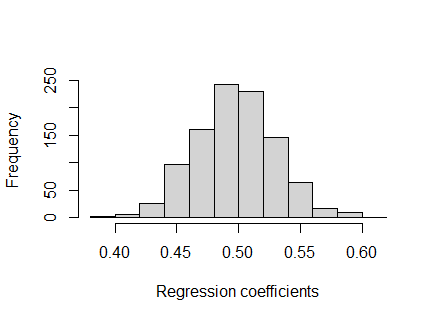
\includegraphics[scale=0.4]{effect of interaction.png}
    \caption{Captain Caption.}
  \end{figure}
\end{frame}

\begin{frame}
  \frametitle{Math examples}
  \begin{equation}
    \hat{H}\Psi = E\Psi
  \end{equation}
  \begin{equation}
    \frac{1}{2}\alpha\beta = \qty|\psi^*\psi|^2
  \end{equation}
\end{frame}

\begin{frame}
  \frametitle{Test block function}
  \begin{block}{Standard Block}
    This is a standard block.
  \end{block}
  
  \begin{exampleblock}{Example Block}
    This is an example block.
  \end{exampleblock}
  
  \begin{alertblock}{Alert Block}
    This is an alert block.
  \end{alertblock}
\end{frame}


\begin{frame}
  % \wider[2cm]{
  \begin{tikzpicture}
    \usebeamertemplate{finalpage}
    \thankyoumessage{Thank you!}
  \end{tikzpicture}
  % }
\end{frame}

\end{document}
